\documentclass[10pt]{article}
\usepackage[letterpaper,textwidth=5.5in,textheight=9in,top=1in]{geometry}
\usepackage{mathptmx}
\usepackage{amsmath}
\usepackage{graphicx}
\graphicspath{{../results/paper/figures/}}
\usepackage{array}
\usepackage[hidelinks]{hyperref}
\IfFileExists{microtype.sty}{\usepackage{microtype}}{}
\setlength{\parskip}{0pt}
\renewcommand{\arraystretch}{1.15}
\clubpenalty=10000
\widowpenalty=10000

% NeurIPS-style headings
\makeatletter
\renewcommand\section{\@startsection{section}{1}{\z@}%
  {-2.0ex \@plus -0.5ex \@minus -0.2ex}{1.3ex \@plus 0.2ex}{\large\bfseries\raggedright}}
\renewcommand\subsection{\@startsection{subsection}{2}{\z@}%
  {-1.6ex \@plus -0.4ex \@minus -0.2ex}{0.7ex \@plus 0.2ex}{\normalsize\bfseries\raggedright}}
\makeatother

\newcommand{\refentry}[1]{\par\noindent\hangindent=1.4em\hangafter=1 {\small #1}\par}

\begin{document}

% ---- Title block ----
\begin{center}
{\LARGE\bfseries The Probe Is the Bottleneck: Zero-Shot Round-Trip Recovery Does Not Yet Certify Emotion Controllability in Text-to-Image Generation\par}
\vspace{14pt}
{\bfseries Urme Bose}
\end{center}
{\let\thefootnote\relax\footnotetext{Code, benchmark, preregistration, and all committed artifacts: \url{https://github.com/urme-b/NovaVision}.}}
\vspace{4pt}

% ---- Abstract ----
\begin{center}\textbf{Abstract}\end{center}
\vspace{-4pt}
\begin{list}{}{\leftmargin=0.4in \rightmargin=0.4in}\item\relax
Round-trip recovery is the default certificate of emotion controllability in text-to-image generation: condition on an emotion, classify the generated image, count the matches. Zero-shot CLIP makes the loop free, and free measurements spread faster than their validation. We test whether this one certifies anything. Our protocol holds image content independent of the intended emotion and bounds every number with a chance floor, a template ceiling, a shuffled-label permutation control, family-wise correction, and probe error deconvolved into the estimate. A CPU pilot (SD-Turbo, CLIP ViT-B/32, $n=14$ per tier) returns a null: no conditioning tier beats the shuffled-label control (Holm-adjusted $p=0.27$), and the emotion tier's apparent lift, 0.214 over a 0.143 chance floor, corrects to 0.165 once the probe's measured error is removed. The null indicts the certificate, not conditioning. In domain the probe collapses onto neutral, using 2 of 7 labels and assigning neutral to 90\% of items; on real scenes it reads emotion at only 40.3\% (ViT-L/14: 45.5\%, McNemar $p=0.038$). We release AffectBench, the harness, and a preregistered powered run ($n=420$ per tier, at least 95\% power) gated on a probe first demonstrating in-domain competence.
\end{list}
\vspace{4pt}

\section{Motivation}
Emotion-conditioned image generation is now a named task with a default metric. EmoGen defined the task and the measurement the field reuses: generate on an emotion, classify the image, count the matches (Yang et al., 2024). EmotiCrafter extended conditioning to continuous valence and arousal (Dang et al., 2025); adapters and guidance followed (Yuan et al., 2025; Xia et al., 2025); training-free prompt conditioning arrived with EPIG (Othmen et al., 2026). The applications are not hypothetical: affective media, accessibility, tools that respond to how a sentence feels rather than what it names. And the stakes are user-facing, because a system that misreads or misrenders affect fails people, not benchmarks.

Every such system faces one question. Did the image convey the emotion, or did we only intend it to? Humans answer slowly and expensively. The round trip answers instantly, and with zero-shot CLIP it answers in one forward pass per image. That cheapness is exactly why the assumption deserves a hard test: a free measurement spreads before anyone checks what it measures. Generative evaluation has been here before. FID contradicts human raters on modern text-to-image models (Jayasumana et al., 2024). Most fidelity metrics fail basic sanity checks (Naeem et al., 2020). No standard metric strongly tracks human judgment at scale (Stein et al., 2023). Emotion round-trip recovery has never received the same scrutiny.

Our claim is narrow by design. We do not show that emotion conditioning fails; we show that this cheap certificate cannot show it succeeds. This paper supplies the missing scrutiny, in runnable form.

\section{Gap}
Three omissions make published round-trip numbers unreadable.

\textbf{No controls.} The field's own metric, Emo-A, classifies generated images with an EmoSet-trained network (Yang et al., 2024) and is reported bare: no chance floor, no template ceiling, no test against random label agreement. Zero-shot variants inherit the bare number and add a second problem, an instrument nobody validated. The failure mode is obvious once stated. If conditioning paints a fixed per-emotion scene and the probe is worded to match it, recovery is a tautology; the number measures prompt-probe vocabulary overlap, not the image.

\textbf{No instrument validation.} The classifier doing the recovering is trusted, not tested. Zero-shot CLIP gets dropped in because it is free, despite image-emotion performance that is weak on abstract art (Widhoelzl et al., 2024) and low enough on standard benchmarks that recent work names the visual affective gap as the problem itself (Wu et al., 2025). No one prints the probe's in-domain error beside the recovery number it produced, and no one propagates that error into the estimate.

\textbf{No preregistration.} Runs are sized and analyzed after the fact. A null becomes indistinguishable from an underpowered shrug; a positive, from a garden of forking paths (Gelman and Loken, 2014).

The metric-critique tradition closed these gaps for FID and Inception Score. For emotion controllability they stand open, and they matter more here: perceived emotion is subtler than fidelity, and the default probe, as Section~5.5 measures, is weaker.

\section{Hypothesis}
The hypotheses are frozen in the repository's preregistration before the powered run. The committed pilot is a calibration of the instrument, not a test of them. All tests are one-sided at $\alpha=0.05$, with Holm correction over the family of three conditioning tiers.

\begin{itemize}\itemsep1pt
\item \textbf{H1 (conditioning beats chance).} For each conditioning tier (naive, emotion, affect), recovery accuracy exceeds the shuffled-label permutation null (2000 permutations).
\item \textbf{H2 (conditioning beats the template).} Each conditioning tier adds recovery over the scene template ceiling, tested as a paired per-item contrast on the content track.
\item \textbf{H0 (the registered null).} Neither holds after multiple-comparison control.
\end{itemize}

One outcome-neutral condition governs all three, in the Registered Reports sense (Chambers, 2013): the probe must demonstrate in-domain competence before any hypothesis test is interpretable. A probe collapsed onto two of seven labels scores chance on balanced data whatever the images show, so a collapsed run is reported as instrument failure, never as evidence for H0.

\section{Research questions}
\begin{itemize}\itemsep1pt
\item \textbf{RQ1.} Does prompt-level conditioning raise recovered-emotion accuracy above the shuffled-label null, per tier, under Holm correction?
\item \textbf{RQ2.} Does any candidate probe clear the registered in-domain gate: more than two of seven labels used on generated scenes, and accuracy above the majority baseline with a confidence interval excluding it? Candidates: CLIP ViT-B/32, ViT-L/14, and an EmoSet-trained classifier through the same interface.
\item \textbf{RQ3.} Does any apparent lift survive Rogan-Gladen correction for the probe's measured error?
\item \textbf{RQ4 (secondary).} On the text track, where valence and arousal are grounded in the sentence rather than a per-emotion prior, does Spearman $\rho$ between intended and recovered affect (with bootstrap CIs) show signal that categorical recovery misses?
\end{itemize}

\section{Methodology}

\subsection{Pipeline and conditioning tiers}
Text enters a DistilRoBERTa emotion classifier (Hartmann, 2022) over seven target labels: anger, disgust, fear, joy, neutral, sadness, surprise (Ekman, 1992). The emotion is grounded in Russell's circumplex (Russell, 1980): valence and arousal come from a per-emotion prior blended with lexical affect from an affect lexicon (empirical norms: Warriner et al., 2013; Mohammad, 2018; the shipped default is a small offline demo) as $v = c\,v_{\mathrm{lex}} + (1-c)\,v_{\mathrm{prior}}$, with lexical coverage $c$ capped at 0.8 so the classifier prior always retains weight; the cap is a stated constant, not a tuned one. Scoring skips function words and applies a two-token negation flip to valence. The blend is a declared heuristic, ablatable at $c=0$ and $c=1$.

Generation is SD-Turbo (Sauer et al., 2023) on a frozen backbone. Conditioning is prompt-level only and increases over the tiers in Table~\ref{tab:tiers}, which are the ablation. Content is never selected by the emotion; the same subject renders under every emotion, and seeds are shared across tiers per item, so contrasts are paired on generation noise.

\begin{table}[t]
\centering\small
\begin{tabular}{l l l}
\hline
\textbf{Tier} & \textbf{Prompt composition} & \textbf{Role} \\
\hline
raw & content + style & negative control, chance floor \\
naive & content + bare emotion word & minimal baseline to beat \\
emotion & content + engineered mood phrase & the method, categorical \\
affect & emotion tier + palette, lighting from $v,a$ & the method, dimensional \\
scene & fixed per-emotion template, no content & positive control, template ceiling \\
\hline
\end{tabular}
\caption{Conditioning tiers. Content is independent of emotion by construction.}
\label{tab:tiers}
\end{table}

\subsection{Recovery and the circularity attack}
A swappable probe reads emotion and graded affect back from the image. The default is CLIP zero-shot (Radford et al., 2021) with two fixes: emotion logits scaled by the model's learned temperature, and valence and arousal taken as expectations over an ordered ladder of anchor prompts at a milder fixed temperature. Probe templates are frozen before measurement at a pinned repository revision and are never tuned on evaluation items.

Circularity, the risk that a CLIP-family probe simply agrees with the emotion word the conditioning wrote, is attacked three ways. Decoupled content forces any signal through the mood modifier, not the depicted scene. The shuffled-label permutation control quantifies the circularity baseline directly: recovery counts only when it clears random target reassignment. And an independent non-CLIP image-emotion probe slots into the same interface, removing the shared vocabulary entirely; validating the headline under it is a prerequisite, not an option.

\subsection{AffectBench}
The content track uses twenty affect-neutral subjects. The text track uses AffectBench, built on demand from GoEmotions (Demszky et al., 2020) under the official Ekman grouping: balanced per-class sampling from the test split (default 100 per class; realized counts logged), exact within-sample dedup, subtraction of any item whose normalized text appears in the train split, counts and a content hash logged, composition and licensing documented in a datasheet (Gebru et al., 2021). GoEmotions is Reddit-English with modest Ekman-level agreement ($\kappa \approx 0.33$ to $0.44$); the benchmark inherits that skew, and the scope is text-prompt controllability, stated as such.

\subsection{Statistics}
Every tier reports recovery accuracy with a bootstrap 95\% CI, macro-F1, valence and arousal correlations with CIs, CLIP-T for content preservation, the majority-class baseline, a probe-collapse diagnostic (how many labels the probe ever uses), and the shuffled-label $p$-value. Holm correction controls the family-wise rate across tiers (Holm, 1979); Cohen's $h$ accompanies every contrast, so significance never travels without magnitude. Because the probe is imperfect, apparent recovery is deconvolved through the Rogan-Gladen estimator (Rogan and Gladen, 1978) using the probe's measured sensitivity and specificity: instrument error becomes a correction, not a caveat.

\subsection{The pilot as proof of concept}
The repository ships a committed CPU pilot (256\,px, 2 subjects, 1 seed; $n=14$ per committed conditioning tier, $n=7$ for scene). Its purpose is calibration: run the protocol end to end and measure the instrument. It did both, and the second finding governs everything.

\begin{table}[t]
\centering\small
\begin{tabular}{l c c c c c}
\hline
\textbf{Tier} & \textbf{Accuracy [95\% CI]} & \textbf{Macro-F1} & \textbf{Shuffled $p$} & \textbf{Holm $p$} & $n$ \\
\hline
raw & 0.143 [0.000, 0.357] & 0.038 & 0.86 & n/a & 14 \\
emotion & 0.214 [0.000, 0.429] & 0.112 & 0.23 & 0.27 & 14 \\
affect & 0.214 [0.000, 0.429] & 0.133 & 0.14 & 0.27 & 14 \\
scene & 0.286 [0.000, 0.575] & 0.184 & 0.14 & n/a & 7 \\
\hline
\end{tabular}
\caption{Pilot recovery by tier. Chance and the majority baseline coincide at 0.143 (1/7). The committed pilot predates the naive tier; a fresh pilot adds it and its contrasts.}
\label{tab:results}
\end{table}

\begin{figure}[t]
\centering
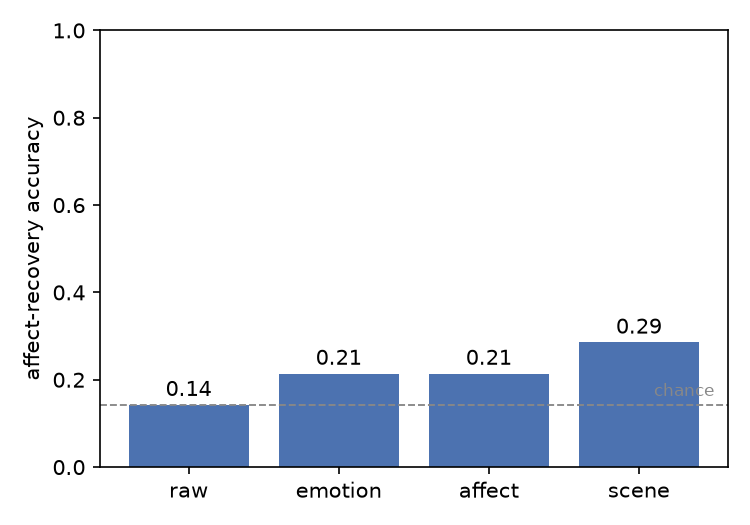
\includegraphics[width=0.58\textwidth]{accuracy.png}
\caption{Recovery accuracy by tier (pilot: SD-Turbo, ViT-B/32, 256\,px; $n=14$ per conditioning tier, 7 for scene). Every interval includes the 1/7 chance line.}
\label{fig:accuracy}
\end{figure}

Read four things together in Table~\ref{tab:results} and Figure~\ref{fig:accuracy}. First, the probe collapsed in domain: 2 of 7 labels used, neutral assigned to 90\% of generated items (Figure~\ref{fig:confusion}). A collapsed probe scores chance on raw by construction, so the floors are necessary but not sufficient; the collapse diagnostic and majority baseline print beside every number for exactly this reason. Second, the lift is one image. Emotion over raw is $+0.071$ (Cohen's $h=0.187$, $p=0.255$), and affect adds nothing over emotion, as expected on the content track, where affect cues are a deterministic function of the emotion prior. Third, no tier clears the shuffled-label control. Fourth, correction sharpens the verdict rather than softening it: the emotion tier's apparent 0.214 becomes 0.165 under Rogan-Gladen, indistinguishable from chance at this $n$, attributing most of the apparent lift to the instrument's error structure.

\begin{figure}[t]
\centering
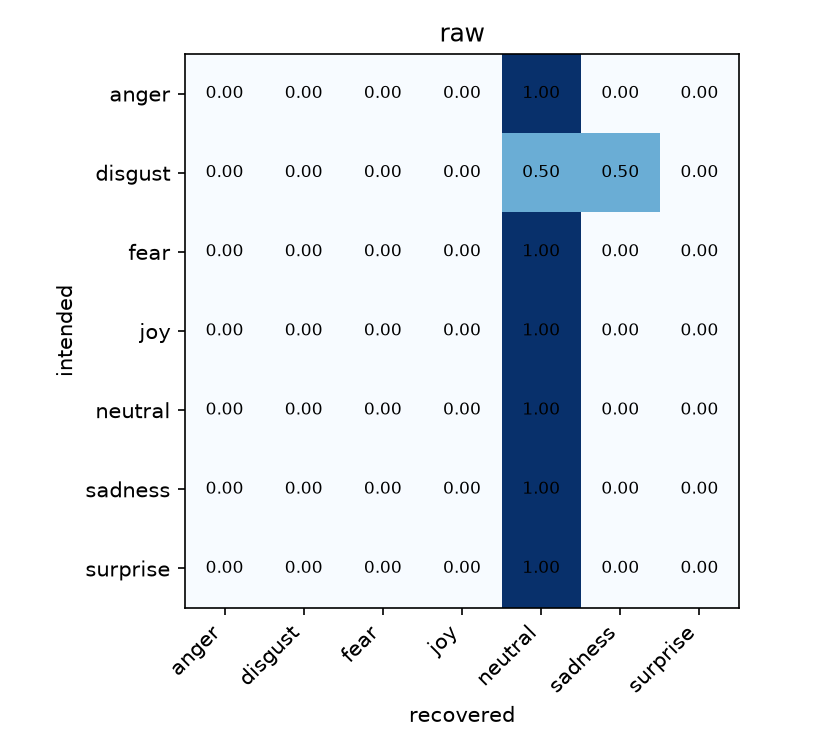
\includegraphics[width=0.42\textwidth]{confusion_raw.png}
\caption{Row-normalized raw-tier confusion from the pilot: predictions collapse onto the neutral column.}
\label{fig:confusion}
\end{figure}

Probe validation locates the failure. Out of domain (faces, $n=200$), ViT-B/32 reads Ekman emotion at 29.0\% (macro-F1 0.22), with bimodal recall: neutral 0.81 and anger 0.61 against surprise 0.04, fear 0.06, sadness 0.08. In domain on real scenes (EmoSet, $n=400$) it reaches 40.3\% while emitting all seven labels; ViT-L/14 reaches 45.5\% (faces: 37.5\%), significant per set by exact paired McNemar test ($p=0.038$ on scenes, discordant 36 vs.\ 57; $p=0.040$ on faces). Two consequences follow. The probes are not blind on real photographs, so the neutral collapse is a property of the generated images (256\,px, 2-step SD-Turbo) interacting with the probe; the generator's affective weakness is a co-suspect. And a structural suspect sits underneath both: image-emotion resources standardize on Mikels' eight categories with no neutral (Mikels et al., 2005; Yang et al., 2023), while the targets here are Ekman plus neutral, and neutral is exactly where the probe collapses.

The pilot did what a Stage~1 calibration should: it proved the harness runs, and it caught its own instrument failing before that instrument could manufacture a conclusion.

\section{Timeline}
The plan is staged as a Registered Report: methods and analysis frozen before the confirmatory data exist (Chambers, 2013; van Miltenburg et al., 2021). Table~\ref{tab:timeline} gives the phases.

\begin{table}[t]
\centering\small
\begin{tabular}{p{0.9cm} p{3.9cm} p{3.9cm} p{3.1cm}}
\hline
\textbf{Phase} & \textbf{Work} & \textbf{Gate to advance} & \textbf{Status} \\
\hline
0 & Build harness, floors, controls; run CPU pilot; commit artifacts & Harness re-derives all numbers in CI & Complete, committed \\
1 & Gate candidate probes in domain: ViT-L/14, then an EmoSet-trained classifier via the probe interface & More than 2 of 7 labels on generated scenes; accuracy above majority with CI excluding it & In progress; L/14 registered candidate (45.5\%, McNemar $p=0.038$) \\
2 & One GPU day: 20 subjects $\times$ 7 emotions $\times$ 3 seeds, $n=420$ per tier (scene 21), 512\,px; frozen analysis of H1, H2, H0 & Stopping rule: one run at registered $n$; no optional stopping, no dropped tiers & Withheld until Phase~1 passes \\
3 & Human study (3+ raters, Cohen's $\kappa$ vs.\ probe); cross-system runs (EmoGen, EmotiCrafter, CoEmoGen) & Rater recruitment; compute & Wired, unrun \\
\hline
\end{tabular}
\caption{Staged plan in Registered Reports form.}
\label{tab:timeline}
\end{table}

Power is fixed before running. At the ViT-L/14 in-domain ceiling of 0.455, $n=420$ per tier gives at least 95\% power to detect even a weak conditioning effect (strength 0.2, recovery 0.205) at $\alpha=0.05$; a Phase~2 null is therefore a properly powered null. If the gated probe collapses in domain, the run is withheld and the probe replaced, not reinterpreted. Deviations are logged in the preregistration before the numbers are read. The result publishes whichever way it comes out.

\section{Contributions}
\begin{itemize}\itemsep1pt
\item \textbf{A gated, preregistered round-trip protocol} for emotion controllability: decoupled content, chance and template floors, a shuffled-label permutation control with Holm correction, effect sizes on every contrast, and probe error deconvolved into the estimate rather than footnoted beside it.
\item \textbf{AffectBench and an open harness}: a frozen, datasheeted, dedup-checked GoEmotions-derived benchmark; pinned models, total run provenance, and a submission schema for scoring any generator or probe under identical rules.
\item \textbf{A diagnosed negative result}: zero-shot CLIP round-trip recovery, as currently practiced, cannot certify emotion controllability. The mechanism is measured, not asserted: in-domain neutral collapse, a 40.3\% ceiling on real scenes, and an apparent lift that correction returns to within noise of chance. The finding warns a subfield off a free metric before it hardens into a leaderboard.
\end{itemize}

\section{Limitations}
The instrument is the binding limitation, and it scopes the central claim: nothing here shows emotion conditioning fails, only that this cheap certificate cannot show it succeeds. A chance-level result is uninformative on its own, since a collapsed probe scores the majority baseline regardless of the image; the collapse diagnostic is reported alongside every number for that reason, and the null is guarded rather than triumphant. Mood modifiers and the CLIP probe share affective vocabulary; the floors bound the leakage and the non-CLIP probe removes it, but that probe's validation is Phase~1 work, not done. On the content track, valence and arousal are per-emotion priors, so the affect-versus-emotion contrast tests palette and lighting only; text-grounded affect is testable only on the text track. The pilot is one generator, one probe, one seed, fourteen items per tier; its intervals span most of the possible range by design, and cross-system claims await Phase~3.

Generated-image quality is a co-suspect: 2-step, 256\,px SD-Turbo may carry little affective signal for any probe to read, a confound the 512\,px powered run reduces but does not remove. AffectBench inherits GoEmotions' Reddit-English domain and modest annotator agreement; disgust is scarce under the Ekman collapse; and the Ekman-plus-neutral taxonomy sits at odds with the Mikels-8 space standard evaluators are trained on. The registered remedy is evaluation on the native taxonomy with an EmoSet-trained probe, the mapping stated rather than hidden. On broader impact: emotion-steered generation, if it worked reliably, would raise manipulation concerns, and a validated measurement protocol is a precondition for auditing such systems, not only for building them. The near-term impact we intend is evaluative: preventing unearned controllability claims.

\section*{Reproducibility statement}
Every model and dataset is pinned to an exact revision, and each run writes a manifest recording git SHA, library versions, device, dtype, and the benchmark content hash. The committed pilot is produced by \texttt{make pilot}; \texttt{make reproduce} is the powered configuration; \texttt{make paper} regenerates the tables and \texttt{make resummarize} the figures from whichever run is present. A continuous-integration target (\texttt{make repro-check}) re-derives all reported numbers from the committed records on every push, and a 200-test suite exercises the deterministic core and the real import path. Cross-device bit-exactness is not guaranteed for diffusion; each run therefore declares its device and dtype in the manifest.

\section*{References}
\refentry{Chambers, C. D. (2013). Registered Reports: A new publishing initiative at Cortex. \emph{Cortex}, 49(3), 609-610.}
\refentry{Dang, S., et al. (2025). EmotiCrafter: Text-to-emotional-image generation based on valence-arousal model. arXiv:2501.05710.}
\refentry{Demszky, D., et al. (2020). GoEmotions: A dataset of fine-grained emotions. \emph{ACL 2020}. arXiv:2005.00547.}
\refentry{Ekman, P. (1992). An argument for basic emotions. \emph{Cognition and Emotion}, 6(3-4), 169-200.}
\refentry{Gebru, T., et al. (2021). Datasheets for datasets. \emph{Communications of the ACM}, 64(12), 86-92.}
\refentry{Gelman, A., and Loken, E. (2014). The statistical crisis in science. \emph{American Scientist}, 102(6), 460-465.}
\refentry{Hartmann, J. (2022). Emotion English DistilRoBERTa-base. Model card, Hugging Face.}
\refentry{Holm, S. (1979). A simple sequentially rejective multiple test procedure. \emph{Scandinavian Journal of Statistics}, 6(2), 65-70.}
\refentry{Jayasumana, S., et al. (2024). Rethinking FID: Towards a better evaluation metric for image generation. \emph{CVPR 2024}. arXiv:2401.09603.}
\refentry{Mikels, J. A., et al. (2005). Emotional category data on images from the IAPS. \emph{Behavior Research Methods}, 37(4), 626-630.}
\refentry{Mohammad, S. M. (2018). Obtaining reliable human ratings of valence, arousal, and dominance for 20,000 English words. \emph{ACL 2018}.}
\refentry{Naeem, M. F., et al. (2020). Reliable fidelity and diversity metrics for generative models. \emph{ICML 2020}, PMLR 119.}
\refentry{Othmen, E., et al. (2026). EPIG: Emotion-based prompting for personalised image generation. arXiv:2606.13247.}
\refentry{Radford, A., et al. (2021). Learning transferable visual models from natural language supervision. \emph{ICML 2021}. arXiv:2103.00020.}
\refentry{Rogan, W. J., and Gladen, B. (1978). Estimating prevalence from the results of a screening test. \emph{American Journal of Epidemiology}, 107(1), 71-76.}
\refentry{Russell, J. A. (1980). A circumplex model of affect. \emph{Journal of Personality and Social Psychology}, 39(6), 1161-1178.}
\refentry{Sauer, A., et al. (2023). Adversarial diffusion distillation. arXiv:2311.17042.}
\refentry{Stein, G., et al. (2023). Exposing flaws of generative model evaluation metrics and their unfair treatment of diffusion models. \emph{NeurIPS 2023}. arXiv:2306.04675.}
\refentry{van Miltenburg, E., van der Lee, C., and Krahmer, E. (2021). Preregistering NLP research. \emph{NAACL 2021}.}
\refentry{Warriner, A. B., Kuperman, V., and Brysbaert, M. (2013). Norms of valence, arousal, and dominance for 13,915 English lemmas. \emph{Behavior Research Methods}, 45, 1191-1207.}
\refentry{Widhoelzl, H., et al. (2024). Decoding emotions in abstract art: Cognitive plausibility of CLIP. arXiv:2405.06319.}
\refentry{Wu, D., et al. (2025). Bridging visual affective gap: Borrowing textual knowledge by learning from noisy image-text pairs. arXiv:2511.17103.}
\refentry{Xia, Y., et al. (2025). MUSE: Manipulating unified framework for synthesizing emotions in images via test-time optimization. arXiv:2511.21051.}
\refentry{Yang, J., et al. (2023). EmoSet: A large-scale visual emotion dataset with rich attributes. \emph{ICCV 2023}. arXiv:2307.07961.}
\refentry{Yang, J., et al. (2024). EmoGen: Emotional image content generation with text-to-image diffusion models. \emph{CVPR 2024}. arXiv:2401.04608.}
\refentry{Yuan, K., et al. (2025). CoEmoGen: Towards semantically-coherent and scalable emotional image content generation. arXiv:2508.03535.}

\end{document}
